\section{\textbf{Introduction}}\label{sec:Introduction}


% ------------------------------------------------------------------------------
% The introduction should lead the reader to the work you've done. You should
% start with general statements and then get close to the core (zoom in). Every
% computer scientist should be able to understand what is paper is about. The
% introduction should follow the same structure as the abstract; but this time
% you should spend one paragraph for each item.
% ------------------------------------------------------------------------------
% ------------------------------------------------------------------------------
% (1) What is the problem? Motivation: broadly, what is problem area,
% why important? Open up the subject (the subject will be electromagnetic
% fields in cylindrical dielectric geometrics, adaptive arrays in packet radio,
% or whatever.)
% Introduce problem, outline the solution; the statement of the problem should
% include a clear statement why the problem is important (or interesting). In
% the case of a conference, make sure to cite the work of the PC co-chairs and
% as many other PC members as are remotely plausible, as well as from anything
% relevant from the previous two proceedings. In the case of a journal or
% magazine, cite anything relevant from last 2-3 years or so volumes. Avoid
% stock and cliche phrases such as "recent  advances in XYZ" or anything
% alluding to the growth of the Internet. Be sure that the introduction lets
% the reader know what this paper is about, not just how important your general
% area of research is. Readers won't stick with you for three pages to find out
% what you are talking about.
% The introduction must motivate your work by pinpointing the problem you are
% addressing and then give an overview of your approach and/ or contributions
% (and perhaps even a general description of your results). In this way, the
% intro sets up my expectations for the rest of your paper -- it provides the
% context, and a preview. Repeating the abstract in the introduction is a waste
% of space.
% ------------------------------------------------------------------------------
%\sidenote{motivation}
%\todotext{One paragraph:What is the problem? What is problem area. Open up the subject.}
Simultaneously to the increasing demands of full connectivity between people and machines, Industrial automation is changing towards matching these enormous growth requirements regarding reliability and latency. It has been progressed through several stages from particular Fieldbus systems over Industrial Ethernet to industrial wireless communication \cite{5535166}. Likewise, the need for continuous connectivity and improved network technologies to meet real-time systems has become critical \cite{Ericsson2019}. The continuous digitalization of the production systems pointed to Industry 4.0. Nevertheless, Industry 4.0 is inspiring the manufacturing area with the provision of decentralized management, control, monitoring and support for real-time systems, giving industrial automation flexibility and making it typical \cite{gardiner2018avnu}\cite{3gpp2018study}. In Consequence, The internet of things (IoT) and machine-to-machine communication (M2M) have been employed to strengthen smart factories in terms of communications and self-monitoring \cite{kagermann2013recommendations}. 
In contrast to the predecessors, 5G is exceptionally beneficial for intelligent manufacturing. It points to support a wide range of vertical industries by appending ultra-reliable low-latency communication(uRLLC), flexibility, and decrease the dependence on cables \cite{Ericsson2019}. 
On the other side, to answer real-time requirements, extra functionalities such as summation frame communication, Time Division Multiple Access (TDMA), or polling-based communication have been included. These additions present rigorous real-time capabilities, but require changes of the original IEEE Ethernet MAC \cite{wisniewski2012fast}. QoS, Timing, synchronization, and resource reservation are some of the promised features by TSN \cite{bello2014novel}.  Nevertheless, the integration of 5G with Time-Sensitive Networking (TSN) has significant advantages: supporting the entire connection in industrial automation, and provide all needed requirements on intelligent factories. To grant satisfactory QoS for end-to-end communication (E2E) in integrated networks \cite{7883994}.
Furthermore, the Integration of 5GC with TSN will be described in three scenarios regarding the distribution of Industrial parts (sensors, actuators, and controllers). Besides, a couple of convenient use cases of integrating 5G mobile networks in the industries area of the future will be covered \cite{3gpp2018study}. Although, ITU classified 5G applications into three types: Enhanced mobile broadband (eMBB), massive machine-type communication (mMTC), and uRLLC shown in figure
\textbf{\ref{fig:IMT_2020_Use-cases}}. At the moment, according to the 3GPP R15 standard, 5G network focuses on eMBB. In order to deploy the 5G architecture, 3GPP defines Non-Standalone (NSA), and Standalone (SA) architectures. You can see the NSA and SA architecture in figure \textbf{\ref{fig:SA_and_NSA_Architecture}}. According to 3GPP release 15 \cite{5G_Tech_Spec_Group_Ser2018study}, 3GPP will release the NSA architecture first. NSA will use the existing 4G infrastructure to deploy the 5G network to support eMBB services. SA is the aim architecture from 3GPP, which will not depend on the 4G infrastructure, will use the 5G radio network, and will afford the eMBB, mMTC, and uRLLC services \cite{Gsma_5G_implguid_study}.
 


\begin{figure}

\centering
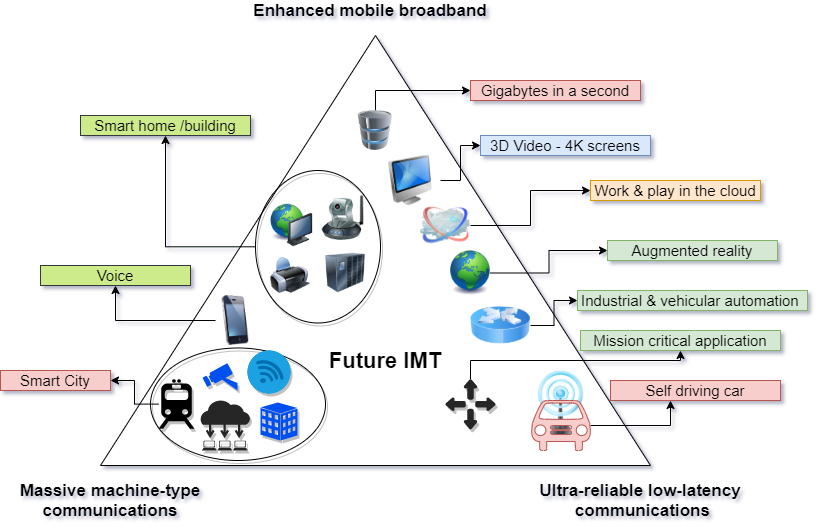
\includegraphics[scale=0.40]{images/IMT_2020_Use-cases.png}
\caption{IMT 2020 Use cases \cite{rancy2016imt}}
\label{fig:IMT_2020_Use-cases}
\end{figure}

In order to reach the topic's goal, we need to dive into the details of 5G Network Architecture; That is, where we have 
Service-based architecture (SBA) outlines the network function (e.g., AMF), and Reference point architecture proves how the Network function services are interacting with the Network function (NF)\cite{5G_Tech_Spec_Group_Ser2018study}.
This paper summarily describes the favorable deployment scenario for an integrated 5G and TSN system in Industry 4.0 field. Additionally, the Integration concepts will clarify the transparent and non-transparent approaches (represented in Tunneling, gateways, and proxies) \cite{ Eri_Gar_Theo_Oper_TSN2017study} \cite{Neumann2018}. \hfill \break
Last but not least, the following chapters will explain the details, including establishing a Protocol Data Unit (PDU) session between ingress TSN Translator (TT) and egress TT over Ethernet, and the required functions that need to be supported by the Open Source 5GC.




\begin{figure}

\centering
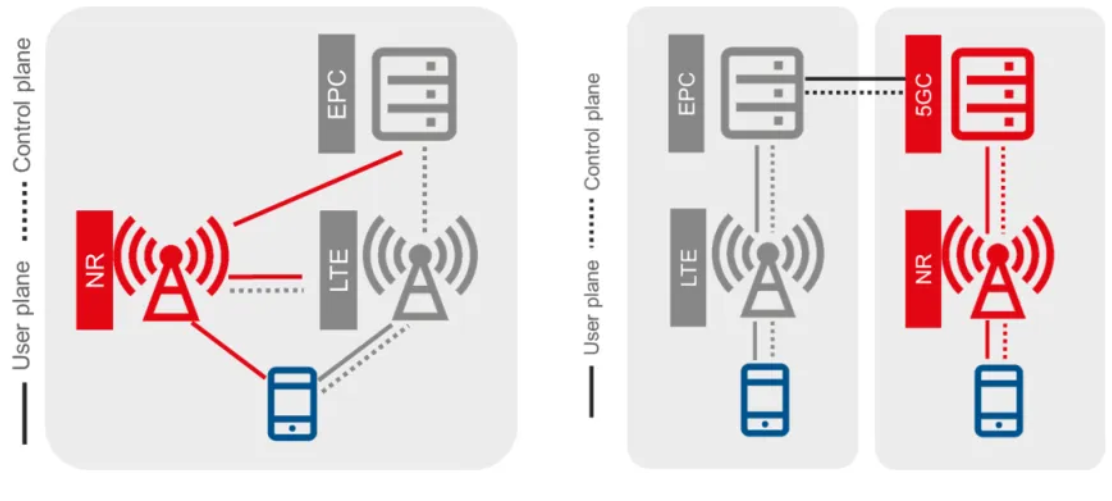
\includegraphics[scale=0.50]{images/SA_and_NSA_Architecture.png}
\caption{SA and NSA  Architecture\cite{Gsma_5G_implguid_study}.}
\label{fig:SA_and_NSA_Architecture}
\end{figure}




 %\hfill \break
 
\section{\textbf{Problem Statement}}\label{Problems} 

\subsection{Reliability and Low Latency}\label{Reliable and Low Latency}

Enhanced mobile broadband (eMBB) term is already in handling in 4G Networks. However,  For 5G, two fundamental classifications have been determined: massive machine-type communication (mMTC) to support an unlimited amount of associated nodes in industrial and consumer fields, and ultra-reliable low-latency communication (uRLLC) for critical communication and correlated control systems \cite{Ginthor2019}.
Figure \textbf{\ref{fig:5G_URLLC_TSN}} depicts the uRLLC features\cite{Ericsson2019}.


The abilities uRLLC empowers 5G to achieve the essential requests of time-sensitive communication, reliability, latency and wireless deterministic. According to the ITU-R\cite{series2017minimum}, Studies and research in 5G networks domain showed that End-to-End reliability is near to 99,999\% and latency of 1 ms of Data packets. However, the data rates higher to many Gb/s, processing entrance for up to a million devices per square kilometer.
5G Networks supports ultra-reliability for control and data channels by providing different techniques, such as encouraging multiple carriers and packet duplication over independent radio links, multi-antenna transmission.

Time-sensitive networking is a collection of Ethernet standards
currently developed by the IEEE 802.1 working group\cite{TSN2019_study}. TSN is an enabler of Industry 4.0 by providing flexible data access and full connectivity for a smart factory. The following reasons support this perspective, but we address them by mentioning and not limiting them. TSN empowers Industrial Automation by performing deterministic communication over Ethernet for real-time applications. By accomplishing scheduled traffic and synchronization, i.e., TSN grants guaranteed latency limitations \cite{Ginthor2019}.
On the other side, in a hybrid network, TSN supports many applications with various QoS requirements, e.g., closed-loop control, to grant the best-effort traffic over an individual standard Ethernet infrastructure\cite{Ericsson2019}. Figure \textbf{\ref{fig:Time-Sensitive_Networking(TSN)Profiles}} draws Time-Sensitive Networking (TSN) features (Selection and Use of TSN tools).



\begin{figure}

\centering
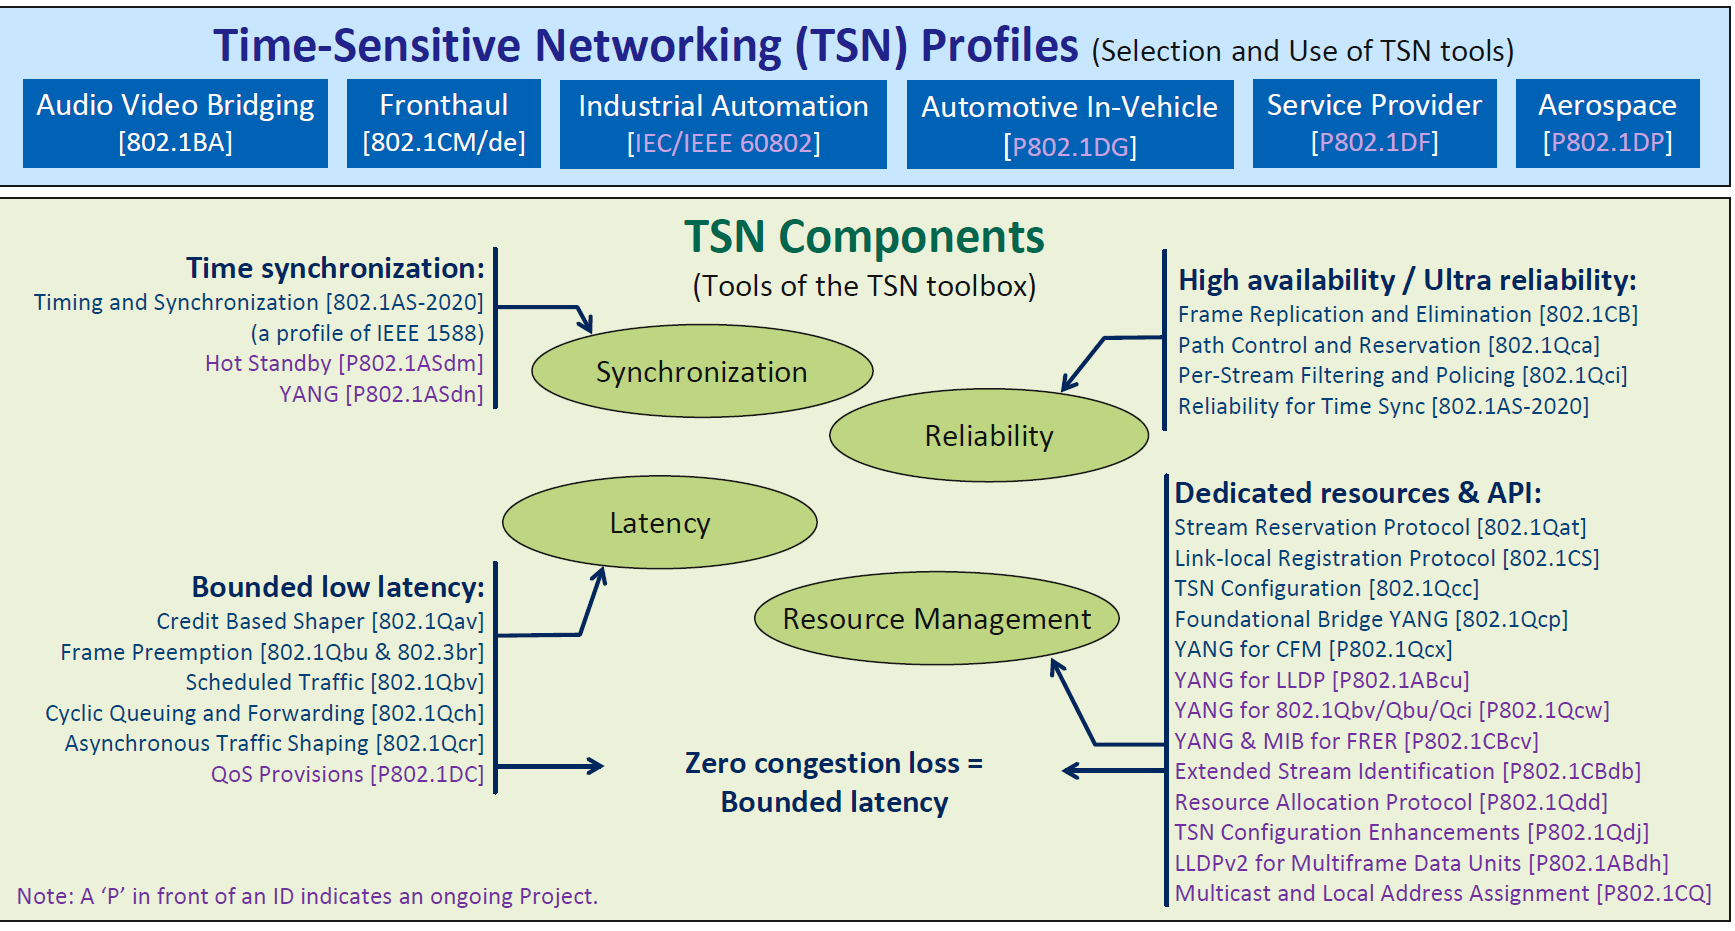
\includegraphics[scale=0.30]{images/Time-Sensitive_Networking(TSN)Profiles.png}
\caption{Time-Sensitive Networking (TSN) Profiles \cite{TSN2019_study}.}
\label{fig:Time-Sensitive_Networking(TSN)Profiles}
\end{figure}



\subsection{Real-Time (Wireless) Communications}\label{Real-Time (Wireless) Communications}
 
  %\hfill \break
  
 Wired networks have always played a primary role in industrial automation. However, the advantages and high efficiency of wireless communication demonstrated by performance indicators in smart manufacturing made it very attractive. Not only in the case of reducing energy consumption, expanding the range and increasing the bandwidth, but also in limiting packet collision. All this gives wireless networks flexibility and mobility. Nevertheless, the most significant factor for real-time systems is preventing collisions and thus ending data packets lost \cite{ring2012wireless}.
On the other hand, some applications like closed-loop control have a demand of periodic uRLLC, or uRLLC with a high refresh rate. This confirms that Synchronous and Hybrid Architecture for Real-Time (RT) Performance (SHARP) is the ideal solution. Which includes both required features uRLLC and Best-Effort traffic \cite{Seijo2019}. Therefore, the trend towards hybrid communication network systems was observed in the past and will continue into the future.
To address Real-Time (Wireless) Communications problems in industrial networks, previous mobile network generations and 5G cellular radio systems include Time synchronization as a fundamental element of their operation. Besides, the wireless network parts themselves are also time-synchronized, e.g., during the precision time protocol telecom profile \cite{ITU_TG82751_study}. All those features make it a strong candidate for time-critical systems. Figure\textbf{\ref{fig:5G_URLLC_TSN}} illustrates uRLLC features. There is a close relation between reliability and time synchronization, i.e., the draw reviews that 5G uses time synchronization for its operations, the multiple antennas, and radio channels that afford reliability\cite{Ericsson2019}. 5G also offers promising ideas and methods for managing low latency and resources, which can be combined to provide superior reliability and low latency.
What arouses curiosity; the 5G system (5GS) also contributes solutions in the core network (CN) for Ethernet networking and URLLC. The 5G CN offers native Ethernet protocol data unit (PDU) sessions. 5G assists in establishing unnecessary user plane paths through the 5GS, including RAN, the CN, and the carrier network. 5GS also allows for a redundant user plane separately between CN and RAN nodes and between the UE and the RAN nodes  \cite{Mannweiler2020}.



%%context

% ------------------------------------------------------------------------------
% (2) Why is it interesting and important? Why is it hard? (e.g., why do
% naive approaches fail?) Narrow down: what is problem you specifically
% consider? Describe the problem addressed in this paper.
% ------------------------------------------------------------------------------
%%\sidenote{importance}

% ------------------------------------------------------------------------------
% (3) Survey past work relevant to this paper. Why hasn't it been solved
% before (related work)? Or, what's wrong with previous proposed solutions? How
% does mine differ?
% ------------------------------------------------------------------------------
%%\sidenote{related work}
%%\todotext{One paragraph: Survey past work relevant to this paper. Why hasn't it been solved before (related work)? Or, what's wrong with previous proposed solutions? How does mine differ?}%%work

% ------------------------------------------------------------------------------
% (4) Define the own approach.
% ------------------------------------------------------------------------------
%%\sidenote{own approach}
%%\todotext{One paragraph: What is the own approach.}%%approach

% ------------------------------------------------------------------------------
% (5) What are the key components of my approach and results? Also include any
% specific limitations. It's the most crucial paragraph, tell
% your elevator pitch: How is it different/better/relates to other work?
% Help the reviewer to get the scientific surplus value between all
% the motivation and basics.
% ------------------------------------------------------------------------------
%%\sidenote{contribution}
%%\todotext{One paragraph: What is the surplus value of this paper.}%%result

% ------------------------------------------------------------------------------
% (6) How have we validated our results?
% ------------------------------------------------------------------------------
%%\sidenote{evaluation}
%%\todotext{One paragraph: How have we validated our results?}%%evaluation

% ------------------------------------------------------------------------------
% (7) How could this work be extended?
% ------------------------------------------------------------------------------
%%\sidenote{outlook}
%%\todotext{One paragraph: ow could this work be extended?}%%outlook

% ------------------------------------------------------------------------------
% (8) ``The remainder of this paper is structured as follows...''. The last
% section must give an overview of the paper.
% ------------------------------------------------------------------------------
% ------------------------------------------------------------------------------
 
 
 
 